\documentclass[10pt, a4paper]{article}
\usepackage[bottom=1.5cm, right=1.5cm, left=1.5cm, top=1.5cm]{geometry}
\usepackage{titlesec}
\usepackage{supertabular}
\usepackage{listings}
\usepackage{wrapfig,lipsum,booktabs}
\usepackage[table,xcdraw]{xcolor}
\usepackage{etoolbox}
\usepackage{amsmath}
\usepackage{hyperref}


\usepackage{graphicx} % for including images
\usepackage{float} % for H float specifier


\title{\textbf{VShooter}}
\author{Gio Carlo Ciudadano \and Rene Andre Jocsing \and Ron Gerlan Naragdao \and Chancy Ponce de Leon}
\date{April 2024}

\begin{document}
\maketitle


	\section{Overview}

	VShooter is a single player top-down rougelite arcade style shooter inspired by Into the Dead, Soul Knight, and frustrating mobile ads for shooters that don't exist (as far as we know). Vshooter blends modern VTuber craze and classic gameplay, aiming for a PG-13 audience and a Windows platform backed by the Unity engine.

  	\section{Gameplay}

	VShooter's gameplay is intuitive. Players select from a pool of VTubers at the start of the game. With their VTuber of choice, players shoot at enemies on a stage. Enemies behave in a variety of ways. They may rush at the player. They may also shoot at the player or exhibit other behaviors. Enemies become progressively more challenging as the player progresses through stages. To offset the increase in difficulty, the player's VTuber maintains an experience bar and gains levels. Experience is gained when an enemy is detroyed. Levels are gained after sufficient experience. Upon gaining a level, the player may select an upgrade for their VTuber, conferring additional properties to the VTuber. VTuber upgrades carry over across stages, but reset upon defeat. Each stage features a boss that the player has to defeat to progress to the next stage.

	\section{VTuber Selection}

	At the start of the game, the player is taken to the VTuber selection screen. They may select a VTuber that they'll control in the game. The VTuber selection screen displays a description of each VTuber available, allowing the player to make an informed decision according to their preferences.
  	
  	\subsection{VTuber Stats} \label{Player Stats}
  	
  	All VTubers have a defined set of base stats.
  	
  	\subsubsection{Primary Stats}

  	\begin{itemize}
  	\item \textbf{Health.} The lose condition of the player controlling the VTuber. All VTubers begin with 500 Health. Health is lost upon collision with enemies or enemy projectiles, or scripted in-game events. If the VTuber's health drops to 0, they lose the game. Lost health may be regained via several types of upgrades (e.g. \textit{lifesteal}, \textit{health regen}, etc.). A VTuber's maximum health may also be increased through upgrades.

  	\item \textbf{Experience.} Defeating an enemy grants experience according to its type. For specifics, please refer to section \ref{Enemies}. 
  	
  	\item \textbf{Level.} If the VTuber gains a set amount of experience, they gain a level. All VTubers begin with 0 experience. The experience required for gaining a level is calculated using the following formula:
  	
  	\[E(L) = 2.5L^2 + 32.5L + 40\]
  	
  	where $L$ is the next level of the VTuber and $E(L)$ is the total experience required to reach the next level.
  	
  	Each additional level requires more experience to be gained. Gaining a level allows the player to select an upgrade from a randomly selected pool. The pool of upgrades are unique for each VTuber. Upgrades can also be upgraded, increasing their potency. For specifics, please refer to section \ref{Upgrades}.
  	
  	\item \textbf{Attack.} Increases the damage dealt by the VTuber's projectiles. All VTubers begin with 20 Attack. Attack may be increased through upgrades.

  	\item\textbf{Defense.} Reduces the total damage received by the VTuber. Additional defense may be gained through upgrades. All VTubers begin with 50 Defense. Defense has reduced effectiveness at higher values. The total damage reduced by defense is calculated using the following formula:
  	
  	\[P_1(x) = P_0(x) \times \frac{100}{100+D}\]
  	
  	where $P_0(x)$ is the pre-mitigation damage, $D$ is the defense of the VTuber, and $N(x)$ is the post mitigation damage.
  	
  	\end{itemize}
  	
  	\subsubsection{Secondary Stats}
  	
  	\begin{itemize}
  	 \item \textbf{Crit Rate and Crit Damage.} Projectile attacks have a chance to deal increased damage to enemies. The chance for a projectile to deal critical damage is determined by the VTuber's \textit{Crit Rate}. The critical damage is determined by the VTuber's \textit{Crit Damage}. All VTubers begin with 0\% Crit Rate and 150\% Crit Damage. Crit Rate and Crit Damage may be increased through upgrades. The total damage is given by the following formula:

  	 \[
	  	 P_0(x) = Rand\begin{cases}
	  	 	R(x) & 1 - C_R\\
	  	 	R(x) \times C_D & C_R \\
	  	 \end{cases}
  	 \]
  	 
  	 where $R(x)$ is the raw damage from the source, $C_R$ is the Crit Rate of the player, $C_D$ is the Crit Damage of the player, and $P_0(x)$ is the (pre-mitigated) damage.
  	 
  	\end{itemize}
  	
  	\subsection{Upgrades} \label{Upgrades}
	
  	\subsubsection{Vtuber Passives}
  	
  	\textit{Vtuber Passives} are sets of three (3) upgrades unique to each VTuber. Vtuber Passives may be upgraded up to three (3) times. For more information on each Vtuber's's Vtuber Passives, please refer to section \ref{VTubers}.
  	
  	\subsubsection{Equipment}
  	
  	\textit{Equipment} are upgrades that are available for all VTubers. Common Equipment may be upgraded up to five (5) times.
  	
  	\begin{center}
		\begin{supertabular}{|p{2.7cm}|p{6cm}|}
			\hline
			\textbf{Name} & \textbf{Description} \\
			\hline
			\textit{\textbf{Iron Sword}} & Increases total attack by 20/30/40/50/60\%. \\
			\textit{\textbf{Heart Gem}} & Increases base health by 50/100/150/200/250. Increases base health regeneration by 2/4/6/8/10HP per second. \\
			\textit{\textbf{Iron Armor}} & Increases defense by 30/60/90/120/150. \\
			\hline
		\end{supertabular}
	\end{center}

	\subsection{VTubers} \label{VTubers}
  	
  	\subsubsection{Mori Calliope}
  	
  	\textbf{Description.} As the Grim Reaper's first apprentice, Mori Calliope specializes in using \textit{lifesteal} and \textit{post death effects} to gain an advantage in battle.
  	
  	\begin{center}
		\textbf{VTuber Passives}
	\end{center}
	
	\begin{center}
		\begin{supertabular}{|p{2.7cm}|p{6cm}|}
			\hline
			\textbf{Name} & \textbf{Description} \\
			\hline
			\textit{\textbf{Soul Harvester}} & Defeating an enemy has a 30/40/50\% chance to restore 20/30/40HP. \\
			\textit{\textbf{Taste of Death}} & Defeating an enemy has a 15/20/25\% chance to create an explosion, dealing 60/80/100 damage. Non-boss enemies caught in the explosion have a 8/10/12\% chance of being immediately destroyed. \\
			\textit{\textbf{End of A Life}}  & Attacks apply [Burn] that deals 15/25/35 damage over 3 seconds. While under the effects of [Burn], targets that fall below 8/12/15\% of their maximum health are immediately destroyed. \\
			\hline
		\end{supertabular}
	\end{center}
	
	\begin{center}
		\textbf{VTuber Actives}
	\end{center}
	\begin{center}
		\begin{supertabular}{|p{2.7cm}|p{6cm}|}
			\hline
			\textbf{Name} & \textbf{Description} \\
			\hline
			\textit{\textbf{Skill 1 (Q)}} & Mori Calliope hurls her scythe forward. Enemies caught in the scythe's path take damage. \\
			\textit{\textbf{Skill 2 (E)}} & Mori Calliope whirls her scythe. Enemies in a small radius around her take damage. \\
			\hline
		\end{supertabular}
	\end{center}
  	
  	\subsection{Enemies} \label{Enemies}

	VShooter features varied enemies for the player to overcome.

	\subsubsection{Deadbeat}

	\begin{figure}[H]
		\centering
		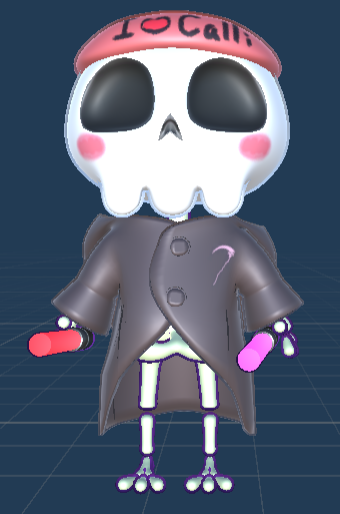
\includegraphics[width=0.5\textwidth]{images/deadbeat1.png}
		\caption{Deadbeat}
		\label{fig:deadbeat}
	\end{figure}
	
	\textbf{Description.} The most common enemy type in the game. These enemies rush toward the player's VTuber. On collision, they explode and deal a small amount of damage.

	\goodbreak

	\subsubsection{Smol Calli}

	\begin{figure}[H]
		\centering
		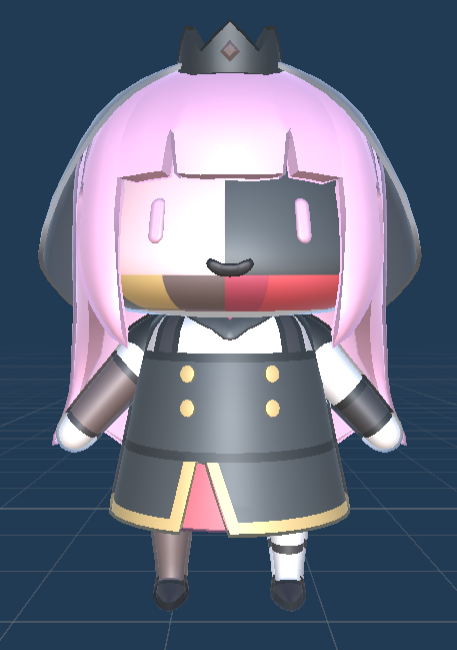
\includegraphics[width=0.5\textwidth]{images/smol_calli1.png}
		\caption{Smol Calli}
		\label{fig:smolcalli}
	\end{figure}

	\textbf{Description.} The first ranged enemy type in the game. These enemies carry a homing missile. They launch the missile toward the player's VTuber and follow after it. If Smol Calli or the homing missile collide with the player's VTuber, they each explode and deal a small amount of damage.

	\subsubsection{Meatshield}

	\begin{figure}[H]
		\centering
		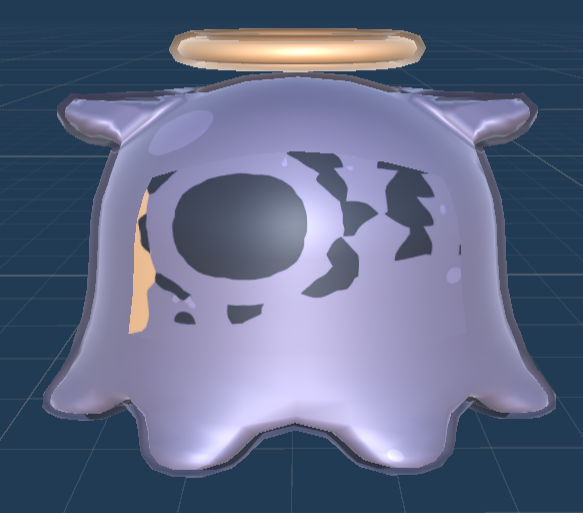
\includegraphics[width=0.5\textwidth]{images/takodachi1.png}
		\caption{Meatshield}
		\label{fig:meatshield}
	\end{figure}

	\textbf{Description.} A slow, bulky enemy characterized by high health. These enemies move in a straight line. They don't go after the player's VTuber, but they deal high damage on collision. Otherwise, they disappear once they move past the edge of the screen.

	\subsubsection{Annoying Healer}

	\begin{figure}[H]
		\centering
		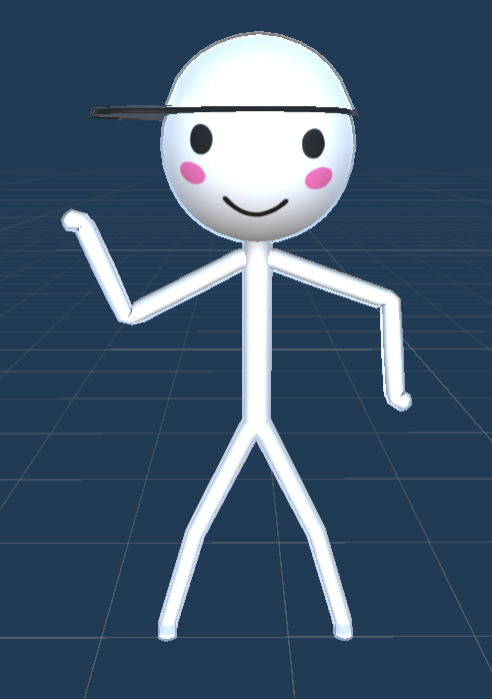
\includegraphics[width=0.5\textwidth]{images/annoying_healer1.png}
		\caption{Annoying Healer}
		\label{fig:annoyinghealer}
	\end{figure}

	\textbf{Description.} A fast and lithe enemy that zips around the stage. These enemies don't go after the player's VTuber nor do they deal damage on collision. However, they recover the health of other enemy types.

\end{document}